% *#06#
%
% imei
% 359 778 047 841 331
%
\renewcommand{\tt}{t}
\newcommand{\yy}{y}
\newcommand{\yn}{{\yy_n}}
\newcommand{\ynn}{{\yy_{n+1}}}
\newcommand{\ta}{a}
\newcommand{\tb}{b}
\newcommand{\tn}{{\tt_n}}
\newcommand{\tnn}{{\tt_{n+1}}}
\newcommand{\zn}{{z_n}}
\newcommand{\znn}{{z_{n+1}}}
\newcommand{\ycero}{{y_a}}
\newcommand{\sol}{\varphi}
\newcommand{\lipschitz}{$y$--Lipschitz\xspace}
\newcommand{\locLipschitz}{localmente \lipschitz}
\newcommand{\globLipschitz}{\lipschitz}
\newcommand{\errCons}{{\cal E}}
\newcommand{\RK}{Runge--Kutta\xspace}
\newcommand{\AB}{Adams--Bashforth\xspace}
\newcommand{\AM}{Adams--Moulton\xspace}

\chapter[Problemas de valor inicial para EDO]
{Problemas de valor inicial para ecuaciones diferenciales de primer
  orden%
  \footnote{\licenseInfo}}

Son muy numerosos los problemas (con orígenes diversos como la física,
química, biología o economía) que se formulan matemáticamente en
términos de ecuaciones diferenciales, es decir, ecuaciones cuya
incógnita, una función $y(x)$, describe un fenómeno dado a través de
una ley que relaciona a esta función con sus derivadas. La formulación
adecuada de esta ley junto a algunos datos adicionales (condiciones
iniciales) garantizarán el buen planteamiento del problema.

Este tema se centra en la resolución numérica de problemas de valor
inicial (o problemas de Cauchy) asociados a ecuaciones diferenciales
ordinarias (EDO). Este tipo de problemas se escriben de la siguiente
forma:
\begin{equation}
  \label{eq:pvi}
  \tag{PVI}
  \left\{
  \begin{aligned}
    &y' = f(\tt,\yy), \quad \tt\in[\ta,\tb],
    \\
    &y(\ta) = \ycero,
  \end{aligned}
  \right.
\end{equation}
donde la función (continua) $f:[\ta,\tb]\times\Rset\to\Rset$ y el
estado inicial $\ycero\in\Rset$ son datos conocidos. En el próximo
tema se estudia el caso general, donde
$f:[\ta,\tb]\times\Rset^n\to\Rset^n$ e $\ycero\in\Rset^n$, con
$n\in\Nset$. En numerosos problemas de la ciencia y la ingeniería, la
variable $\tt$ representa el tiempo aunque no siempre es necesario que
sea así. Con frecuencia hablaremos de $\tt$ como la <<variable
temporal>>).

\begin{definition}
  Llamamos solución de~\eqref{eq:pvi} a toda función $\sol\in
  C^1([\ta,\tb])$ tal que $\sol'(\tt)=f(\tt,\sol(\tt))$ para todo
  $\tt\in[\ta,\tb]$ y además $\sol(\ta)=\ycero$.\label{def:3}
\end{definition}

Obsérvese que, según esta definición, el concepto de solución tiene un
sentido global (en todo el intervalo $[a,b]$), no local (en un entorno
de $\ta$). Como paso previo a la resolución numérica
de~\eqref{eq:pvi}, deberemos garantizar que este problema está bien
planteado, es decir asegurar la existencia y unicidad de solución en
el sentido anterior.

\section{Resultados teóricos preliminares}
\label{sec:tema4:resultados-teoricos}

Antes de comenzar a estudiar métodos numéricos para la resolución de
problemas de Cauchy, recordaremos en esta sección algunos
resultados relacionados con la existencia y unicidad de solución
de~(\ref{eq:pvi}), que resultarán útiles para garantizar existencia de
solución en los problemas que aparecerán en las siguientes secciones.
La clave en estos resultados será el analizar si la función $f(x,y)$
es verifica la condición de Lipschitz que se define a continuación:

\begin{definition}
  \label{def:lipschitz}
  Decimos que una función $f(\tt,y)$ verifica la condición de
  \resaltar{Lipschitz uniformemente} (o globalmente) respecto a $y$ en
    $[\ta,\tb]$ (o simplemente que $f$ es \globLipschitz)
    si existe $L>0$ tal que
  \begin{equation*}
    |f(\tt,y) - f(\tt,z)| \le L |y-z|, \quad \forall \tt\in [\ta,\tb],
    \quad  \forall y,z\in \Rset.
  \end{equation*}
  Decimos que una función $f(\tt,y)$ verifica la condición de
  \resaltar{Lipschitz localmente} respecto a $y$ en
  $[\ta,\tb]$ (o que $f$ es \locLipschitz) si para todo compacto
  $K\subset\Rset$ existe $L_K>0$ tal que
  \begin{equation*}
    |f(\tt,y) - f(\tt,z)| \le L_K |y-z|, \quad \forall \tt\in [\ta,\tb],
    \quad  \forall y,z\in K.
  \end{equation*}
\end{definition}

Fijaremos la siguiente
\textbf{notación}: $\dy f$ designará a la derivada parcial de $f$
respecto a $y$, es decir $\dy f(\tt,y) = \frac{\partial f}{\partial
  \yy}(\tt,y)$. Para el resto de las variables se usarán notaciones
similares.
\begin{remark}
  En la práctica, para estudiar si una función es (local o
  globalmente) Lipschitz se suelen usar las siguientes condiciones
  suficientes:
  \begin{enumerate}
  \item Si $\dy f$ es continua en $[\ta,\tb]\times\Rset$, entonces $f$
    es \locLipschitz.
  \item Si además $\dy f$ está acotada en
    $[\ta,\tb]\times\Rset$, entonces $f$ es uniformemente
    \globLipschitz.
  \end{enumerate}
  Comprobaremos la segunda de estas afirmaciones (la primera se
  demuestra de forma análoga, usando que $\dy f$ está acotada
  en todo compacto $K\subset\Rset)$.
  Si $\dy f$ es continua en $[\ta,\tb]\times\Rset$, entonces en cada
  <<instante>> $t\in[\ta,\tb]$ la función
  $$\dy f(t,\cdot):\Rset \to \Rset$$
  es continua. Aplicando el teorema del valor medio, se tiene que
  dados $y$, $z\in\Rset$ existe $y^*$ entre $y$ y $z$ tal que
  \begin{equation*}
    |f(\tt,y)-f(\tt,z)| = |\dy f(\tt,y^*) \cdot (y-z)|.
  \end{equation*}
  Como además  $\dy f$ está acotada, existe $L>0$ tal que $|\dy
  f(\tt,y)|\le L$ para todo $(\tt,y)\in [\ta,\tb]\times\Rset$ y
  entonces
  \begin{equation*}
    |f(\tt,y) - f(\tt,z)| \le L |y-z|.
  \end{equation*}
\end{remark}

% \begin{example}
%   La función $$f(x,y)=y^2$$ es \locLipschitz en cualquier intervalo
%   $[\ta,\tb]$, pues su derivada parcial $\dy f(x,y)=2y$ es continua. Sin
%   embargo, esta función no está acotada cuando $y\in\Rset$, por lo que
%   no tenemos garantías de que $f(x,y)$ sea uniformemente \globLipschitz.

%   Veamos que realmente $f(x,y)$ no es a uniformemente \globLipschitz,
%   comprobando que para cualquier constate $L>0$, podemos encontrar dos
%   valores, $y_L$, $z_L\in\Rset$ de forma que
%   \begin{equation*}
%   |f(\tt,y_L)-f(\tt,z_L)| >  L  |y_L-z_L|.
%  \end{equation*}
%  Por ejemplo, dada $L>0$ podemos tomar $y_L=L$ y $z_L=0$, así el
%  primer miembro es
%  \begin{align*}
%    |f(\tt,y_L)-f(\tt,z_L)|&=|L+0|\cdot |L-0|=4L^2,
%    \intertext{mientras que el segundo miembro resulta}
%    L|y_L-z_L|&=2L^2<4L^2.
%  \end{align*}
% \end{example}

Los siguientes teoremas constituyen los resultados teóricos
fundamentales de existencia y unicidad para problemas de Cauchy. El
primero utiliza hipótesis más débiles (\locLipschitz), aunque sin
alcanzar directamente la existencia y unicidad de solución global en
todo $[a,b]$. El Teorema~\ref{thm:existencia-unif-lipschitz} garantiza
la existencia y unicidad de solución de~\eqref{eq:pvi} en $[a,b]$,
aunque a costa de imponer una hipótesis muy fuerte (Lipschitz
uniforme), que reduce considerablemente el rango de problemas
diferenciales abarcados.
\begin{theorem}
  \label{thm:existencia-loc-lipschitz}
  Sea $f$ continua en $[\ta,\tb]\times\Rset$ y \locLipschitz. Entonces, para
  cualquier inicialización $\ycero\in\Rset$:
  \begin{enumerate}
  \item Existe una única solución local (definida sólo en
    $[\ta,\ta+\varepsilon]$ para algún $\varepsilon>0$) y existe una
    única solución maximal\footnote{Una solución maximal es una
      solución local, $\sol$, de~\eqref{eq:pvi} que
      \begin{itemize}
      \item O bien está definida en todo $[a,b]$ (por tanto es una
        solución global de~\eqref{eq:pvi}).
      \item O bien está definida en $[\ta,c)\subset[\ta,\tb]$, para
        algún $c\in(\ta,\tb)$, y no es prolongable a $\tt>c$.
      \end{itemize}}
    de~\eqref{eq:pvi}.
  \item Además: si esta solución maximal $\sol(\tt)$ no está definida en todo
    $[\ta,\tb]$ es porque explota en tiempo finito (es decir existe
    $c\in (\ta,\tb)$ tal que $\lim_{\tt\to c^-} \sol(\tt) = \infty$).
  \end{enumerate}
\end{theorem}

\begin{theorem}[Picard]
  \label{thm:existencia-unif-lipschitz}
  Sea $f$ continua en $C^0([\ta,\tb]\times\Rset)$ y (globalmente) \globLipschitz.
  Entonces, para cualquier inicialización $\ycero\in\Rset$, existe una
  única solución de~\eqref{eq:pvi}, que está definida en todo el
  intervalo $[\ta,\tb]$.% Además, para todo $\tt\in[\ta,\tb]$
  % se tiene la siguiente desigualdad:
  % \begin{equation*}
  %   |y(\tt)-y(\ta)| \le (\tb-\ta) \Big( \max_{\tt\in[\ta,\tb]}
  %     f(\tt,y(\ta))\Big) e^{L(\tt-\ta)}.
  % \end{equation*}
\end{theorem}

En lo que sigue, estudiaremos el análisis numérico de problemas
diferenciales en los que, en principio, la función $f(\tt,y)$ es tan
solo \locLipschitz. Luego el estudio de la existencia de
solución en $[\ta,\tb]$ no será una tarea inmediata. Usando el
Teorema~\ref{thm:existencia-loc-lipschitz}, intentaremos demostrar que
la solución maximal del problema~(\ref{eq:pvi}) está acotada en
$[\ta,\tb]$ y por tanto no explota en tiempo finito en este intervalo,
garantizando así existencia y unicidad de solución en $[\ta,\tb]$ (ver
en el ejemplo~\ref{ex:existencia-unicidad-loc-lipschitz}). Con este
propósito, recordamos ahora algunas propiedades interesantes de las
ecuaciones diferenciales que nos resultarán de gran utilidad.

\begin{proposition}[Algunas propiedades de las soluciones de~(\ref{eq:pvi})]
\label{pro:propiedades-pvi}
  Bajo las hipótesis del teorema~\ref{thm:existencia-loc-lipschitz}
  ($f$ \locLipschitz):
  \begin{enumerate}
  \item Sean $\sol_1(\tt)$ y $\sol_2(\tt)$ las soluciones de dos
    problemas del tipo~\eqref{eq:pvi} para la \textbf{misma ecuación
    diferencial} $y'=f(\tt,y)$ pero con \textbf{distintas condiciones
    iniciales}, es decir:
    $$\sol_1(\ta)<\sol_2(\ta)$$
    Entonces las gráficas de $\sol_1$ e $\sol_2$ no se cortan en
    ningún punto. En concreto, si $\sol_1$ y $\sol_2$ están
    definidas, respectivamente, en los intervalos $I_1$ e $I_2$,
    entonces
    \begin{equation*}
      \sol_1(\tt) < \sol_2(\tt), \quad \forall \tt \in I_1
      \cap I_2.
    \end{equation*}

  \item Sean $\sol_1(\tt)$ y $\sol_2(\tt)$ las soluciones de dos
    problemas del tipo~\eqref{eq:pvi} con la \textbf{misma condición
      inicial} pero con \textbf{ecuaciones diferenciales distintas},
    $y'=f_1(\tt,y)$ $y'=f_2(\tt,y)$. Si
    $$
    f_1(\tt,y) \le f_2(\tt,y) \quad \forall \tt\in[\ta,\tb], \quad
    \forall y\in\Rset,
    $$
    entonces
    $$
    \sol_1(\tt)\le \sol_2(\tt) \quad \forall \tt \in
    I_1 \cap I_2.
    $$
  \end{enumerate}
\end{proposition}

\begin{example}
  \renewcommand{\tt}{x}
  \label{ex:existencia-unicidad-loc-lipschitz}
  Estudiaremos la existencia y unicidad de solución del siguiente
  problema de valor inicial:
  \begin{equation*}
    \left\{
      \begin{aligned}
        &y' = -y^2+2y\,\cos \tt, \quad \tt\in [0,2],\\
        &y(0)=1.
      \end{aligned}
    \right.
  \end{equation*}
  En primer lugar, $f(x,y)=-y^2+2y\,\cos \tt$ y $\dy f(t,y)=-2y+2\cos
  t$ son continuas en $[0,2]\times\Rset$, luego $f$ es \locLipschitz,
  por lo que (según el teorema~\ref{thm:existencia-loc-lipschitz})
  existe una única solución maximal, a la que denominaremos
  $\sol(\tt)$, definida en $I=[0,2]$ o bien en $I=[0,c)$ con
  $c<2$. Pero esta última posibilidad no se verifica, pues entonces
  $\sol(\tt)$ explotaría en $c$, pero veremos a continuación que
  $\sol(\tt)$ está acotada:
  \begin{enumerate}
  \item Sea $\sol_1$ la solución del problema de valor inicial para la
    misma ecuación diferencial pero para la condición inicial
    $y(0)=0$. Está claro que su única solución es $\sol_1(\tt)=0$
    para todo $\tt\in\Rset$. Y como $0=\sol_1(0)<\sol(0)=1$, entonces
    (según la proposición~\ref{pro:propiedades-pvi}, parte 2) podemos
    asegurar que $\sol$ está acotada inferiormente:
    \begin{equation*}
      0=\sol_1(\tt)<\sol(\tt), \quad \forall \tt\in I.
    \end{equation*}
  \item Sea ahora $f_2(\tt,y)=-y^2+2y$. Como $\cos\tt \le 1$  (y como
    ya podemos suponer $y>0$):
    $$f(\tt,y)=-y^2+2y\cos\tt \le -y^2+2y = f_2(\tt,y)\quad
    \forall \tt\in I, \forall y\in\Rset^+.$$
    Ahora podemos calcular
    directamente la solución $\sol_2$ del problema de valor inicial
    $y'=f_2(\tt,y)$, $y(0)=1$ (ya que la ecuación es autónoma),
    obteniendo:
    $$
    \sol_2(\tt)=\frac{2e^{2\tt}}{1+e^{2\tt}},
    $$
    función continua y, en consecuencia, acotada superiormente en $[0,2]$.
    Según la proposición~\ref{pro:propiedades-pvi} (parte 1)
    \begin{equation*}
      \sol(\tt)\le\sol_2(\tt),
    \end{equation*}
    luego $\sol(\tt)$ está también acotada superiormente en
    $[0,2]$. Por lo tanto, $\sol$ está definida en todo $[0,2]$.
  \end{enumerate}
  \renewcommand{\tt}{t}
\end{example}

\section{El método de Euler}

A partir de ahora, nuestro objetivo será la descripción, análisis e
implementación de distintos métodos numéricos para la aproximación de
la solución de~\eqref{eq:pvi}. Estos métodos partirán con la
definición de una partición del intervalo $[\ta,\tb]$, formada por
$N+1$ puntos:
\begin{equation*}
  \ta=\tt_0 < \tt_1 < \cdots < \tt_N=\tb.
\end{equation*}
Por simplicidad, supondremos que la partición es uniforme, es decir,
\begin{equation*}
  \text{ si } h=\frac{b-a}{N}, \quad \text{entonces} \quad
  \tt_n=\ta+n\cdot h,\quad \forall n=0\dots,N
\end{equation*}
(en particular, $\tt_0=a$ y $\tt_N=b$). A continuación procedemos como
sigue:
\begin{enumerate}
\item Usamos el dato inicial $y_a$ para arrancar el método numérico,
  definiendo $y_0=y_a$ (más generalmente, $y_0\approx y_a$)
\item Seguidamente definimos una sucesión de forma que $y_{n+1}$ se
  calcula a partir de $y_n$ (y posiblemente de $y_{n-1}$, ...,
  $y_{n-k}$ para algún $k\ge 1$), con el fin de que
  $y_n\approx\sol(\tn)$.
\end{enumerate}
Nuestro objetivo será que el método sea \textit{convergente}, en el
sentido de que la solución aproximada $\{\yn\}_n$ ``converja a la
solución exacta'' $\{\sol(\tn)\}_n$ cuando $h\to 0$. Íntimamente
relacionados con la convergencia están los conceptos de
``\textit{estabilidad}'' y ``\textit{consistencia}'', que estudiaremos
más adelante.
% \begin{enumerate}
% \item El método es \textit{consistente}, si la solución exacta
%   $\{\sol(\tn)\}_n$ ``verifica aproximadamente'' el esquema
%   numérico
% \item El método es \textit{estable} si ``responde continuamente'' a
%   perturbaciones en los datos iniciales.
% \end{enumerate}
% Más adelante distinguiremos entre métodos de un paso, en los que
% para calcular $y_{n+1}$ utilizamos solamente de $y_n$ y métodos
% multipaso, en los que  $y_{n+1}$ depende de los datos en varias etapas
% anteriores ($y_{n}$, $y_{n-1}$, ..., $y_{n-k}$ para algún $k\ge 1$.)

El método más sencillo es el de Euler (más precisamente, el método
de Euler explícito):
\begin{equation}
  \tag{EU}
  \label{eq:metodo-euler}
  \left\{
    \begin{aligned}
      &y_0 = \ycero, \\
      &y_{n+1} = \yn + h f(\tn, \yn), \quad n=0,\dots,N-1.
    \end{aligned}
  \right.
\end{equation}

Este método admite varias interpretaciones:

\subsection*{Interpretaciones del método de Euler}

\subsubsection*{Interpretación geométrica}
En la ecuación $y(\tt)'=f(\tt,y(\tt))$ se puede interpretar que
$f(\tt,y(\tt))$ marca la pendiente (la derivada) de la solución,
$\sol(\tt)$ en cada instante $\tt\in [\ta,\tb]$.

\begin{center}
  \begin{graficaTikz}[width=23em, height=17em]
    \begin{axis}[ \axisXYmiddle, xtick=\empty, ytick=\empty, legend
      pos = north east, xlabel=$t$ ]
      % Draw a curve
      \addplot[domain=1.3:3.3, blue, ultra thick] {20+x*x*x*x};
      \addplot[domain=1.5:3.1, red, thick] {36+32*(x-2)};
      % Plot a label at curve root
      \node[coordinate, medium dot,
      pin={[fill=blue!10!white]120:{\scriptsize $\sol(\tn)$}}] at
      (axis cs:2,36) {};
      \node[coordinate, medium dot, blue,
      pin={[fill=blue!10!white]120:{\scriptsize $\sol(\tt_{n+1})$}}] at
      (axis cs:2.7,73.144) {};
      % \node[coordinate, medium dot, blue, pin=100:{\scriptsize
      % $\sol(\tt_{n+1})$}] at (axis cs:2.7,73.144) {};
      \addplot[dashed] coordinates {(2,7) (2,36)};
      \addplot[dashed] coordinates {(2.7,7) (2.7,58.4)};
      \node[coordinate, medium dot, pin=-30:{$y_{n}$}] at
      (axis cs:2,36) {};
      \node[coordinate, medium dot, pin=-30:{$y_{n+1}$}] at
      (axis cs:2.7,58.4) {};
      % Draw the name of curve
      \legend {$y(t)$};
    \end{axis}
  \end{graficaTikz}
\end{center}

Luego, suponiendo que $\yn$ es una buena aproximación de
$\sol(\tn)$ (por simplificar, $\yn=\sol(\tn)$):
\begin{enumerate}
\item Calculamos la recta, $r$, que pasa por $(\tn,\yn)$ y tiene pendiente
  $f(\tt_n, \yn)$:
  $$
  r(\tt) = \yn +  f(\tt_n, \yn) (\tt-\tt_n).
  $$
\item Calculamos $y_{n+1}$ como la ordenada de esta recta en
  $\tt=\tt_{n+1}$ es decir:
  $$
  y_{n+1} = r(\tt_{n+1}) =
  \yn +  f(\tt_n, \yn) (\tt_{n+1}-\tt_n) = \yn +  f(\tt_n, \yn) \cdot h.
  $$
\end{enumerate}
Así obtenemos el método~\eqref{eq:metodo-euler}.

\subsubsection*{Desarrollo de Taylor}

Suponiendo que $\sol(t)$ (la solución exacta de~(\ref{eq:pvi})) es de
$C^2([\ta,\tb])$, podemos hacer su desarrollo de Taylor en $\tn$:
\begin{equation*}
  \sol(\tnn)=\sol(\tn+h) = \sol(\tn) + h\sol'(\tn) + \frac{h^2}{2} y''(\xi),
\end{equation*}
donde $\xi\in(\tn,\tnn)$. Como $\sol''$ está acotada, el último
término (el resto) será despreciable cuando $h$ es suficientemente
pequeño (pues contiene el factor $h^2$):
\begin{align}
  \label{eq:euler.taylor.1}
  \sol(\tnn)&\approx \sol(\tn) + h\sol'(\tn),
              \intertext{es decir,}
              \notag
              \sol(\tnn)&\approx \sol(\tn) + h f(\tn,y(\tn)),
                          \intertext{y aproximando $\sol(\tn)\approx \yn$, $\sol(\tnn)\approx\ynn$:}
                          \notag
                          \ynn &\approx \yn + h f(\tn,\tn).
\end{align}

\paragraph{Notación.}
Para cualquier sucesión $\{y_n\}_n$, se utilizará la siguiente
notación para el cociente incremental (derivada discreta o diferencia
finita retrógrada de $\ynn$):
\begin{equation}
  \label{eq:derivada-discreta}
  \ddt\ynn = \frac{\ynn-\yn}{h}.
\end{equation}
Así el método de Euler se puede escribir como
\begin{equation*}
  \ddt\ynn = f(\tn,\yn).
\end{equation*}

Utilizando diferentes formulaciones de la derivada discreta, se podrían
haber expuesto ahora algunas variantes del método de Euler, pero éstas
serán introducidas a través de fórmulas de integración.

\subsubsection*{Integración numérica}
La solución exacta de~(\ref{eq:pvi}) puede escribirse de la siguiente
forma (formulación integral de la solución de~(\ref{eq:pvi})):
\begin{equation*}
  \sol(t) = \sol(\ta) + \int_\ta^t f(s,\sol(s))\, ds.
\end{equation*}
La formulación anterior sigue siendo válida si sustituimos $a$ por cualquier otro punto de $[a,b]$. En particular, para
$a=\tn$ y< $t=\tnn$:
\begin{equation}
  \label{eq:tema4.5}
  \sol(\tnn) = \sol(\tn) + \int_\tn^\tnn f(s,\sol(s))\, ds.
\end{equation}
Para obtener el método de Euler implícito aproximamos la última
integral mediante la siguiente fórmula de cuadratura (regla
rectangular izquierda):
\begin{equation*}
  \int_a^b g(s)\,ds \approx hg(a), \quad \text{ con $h=b-a$}.
\end{equation*}
Aplicándola en el intervalo $[\tn,\tnn]$ para la formulación integral
anterior,
\begin{equation*}
  \ynn =  \yn + h f(\tn,\yn),
\end{equation*}
con $\yn\approx\sol(\tn)$, $\ynn\approx\sol(\tnn)$.

\subsubsection*{Algunas variantes del método de Euler.}

Utilizando otras fórmulas de cuadratura, para aproximar la integral
$$\int_\tn^\tnn f(s,\sol(s))\, ds$$ en~(\ref{eq:tema4.5}),<
se obtienen métodos numéricos
distintos al de Euler explícito. Por ejemplo:
\begin{enumerate}
\item Aproximando $\int_\tn^\tnn f(s,\sol(s))\, ds$ por la regla
  rectangular derecha,
  \begin{equation*}
    \int_a^b g(s)\,ds \approx hg(b)
  \end{equation*}
  se obtiene el \textit{Método de Euler implícito}:
  \begin{equation}
    \label{eq:euler-implicito}
    \tag{EI}
    \left\{
      \begin{aligned}
        &y_0=\ycero,\\ &\ynn = \yn + h f(\tn,\ynn).
      \end{aligned}
    \right.
  \end{equation}
  El método anterior se dice \textit{implícito} porque, en general,
  $\ynn$ no puede calcularse explícitamente, pues aparece en el
  segundo miembro. Sin embargo, este tipo de métodos tienen buenas
  propiedades desde el punto de vista de la estabilidad y existen
  casos particulares muy interesantes (por ejemplo, el caso $f$ es
  lineal) en el que los métodos implícitos son muy usados.

\item Aproximando $\int_\tn^\tnn f(s,\sol(s))\, ds$ por la regla del
  punto medio (que tiene orden mayor que las reglas rectangular
  derecha e izquierda):
  \begin{equation*}
    \ynn = \yn + h \; f(\tt_{n+1/2},\sol(\tt_{n+1/2})).
  \end{equation*}
  \begin{enumerate}
  \item Si aproximamos seguidamente $\sol(\tt_{n+1/2})$ por
    $\frac12\big(\sol(\tn)+\sol(\tnn)\big)$, se tiene el siguiente
    método implícito, conocido como método de \textit{Crank-Nicolson}
    (primera versión):
    \begin{equation}
      \label{eq:crank-nicolson-1}
      \tag{CN$_1$}
      \left\{
        \begin{aligned}
          &y_0=\ycero,\\
          &\ynn = \yn + h \; f\big(\tt_{n+1/2},\; \frac{\yn+\ynn}{2}\big).
        \end{aligned}
      \right.
    \end{equation}
  \item El método anterior es implícito y por tanto (en general) no
    puede aplicarse directamente. Pero si aproximamos $\sol(\tt_{n+1/2})$
    por $\sol(\tn)+\frac{h}{2}f(\tn,\sol(\tn))$ se llega al método
    explícito conocido como de \textit{Euler--Cauchy}, del
    \textit{punto medio} o \textit{Euler modificado}:
    \begin{equation}
      \label{eq:euler-cauchy}
      \tag{EC}
      \left\{
        \begin{aligned}
          &y_0=\ycero,\\
          &\ynn = \yn + h \; f\big(\tt_{n+1/2},\;
          \yn+\frac{h}{2}f(\tn,\yn) \big).
        \end{aligned}
      \right.
    \end{equation}
  \end{enumerate}
\item Si aproximamos $\int_\tn^\tnn f(s,\sol(s))\, ds$ por la regla
  del trapecio se llega al siguiente método implícito (segunda
  variante del método de Crank-Nicolson):
  \begin{equation}
    \label{eq:crank-nicolson-2}
    \tag{CN$_2$}
    \left\{
      \begin{aligned}
        &y_0=\ycero,\\
        &\ynn = \yn + \frac h2 \; \big\{f(\tn,y_n))+f(\tnn,y_{n+1})\big\}.
      \end{aligned}
    \right.
  \end{equation}
  Si además aproximamos $\sol(\tnn)$ por
  $\sol(\tn)+hf(\tn,\sol(\tn))$ se llega al método explícito
  conocido como de \textit{Euler mejorado} (o \textit{método de Heunn}):
  \begin{equation}
    \label{eq:euler-mejorado}
    \tag{EM}
    \left\{
      \begin{aligned}
        &y_0=\ycero,\\
        &\ynn = \yn + \frac{h}{2} \; \left\{ f(t_n,y_n) + f\big(\tnn,\;
        \yn+h f(\tn,\yn) \big)  \right\}.
      \end{aligned}
    \right.
  \end{equation}
\end{enumerate}
Estos métodos numéricos se pueden escribir en una notación
algo más sencilla (y más cercana a la ecuación diferencial original),
utilizando la derivada discreta definida
en~\eqref{eq:derivada-discreta}. Por ejemplo, el método de Euler
implícito~\eqref{eq:euler-implicito} se sintetiza en:
\begin{equation*}
  y_0=\ycero,\quad \ddt\ynn = f(\tnn,\ynn).
\end{equation*}


\section{Error y convergencia en el método de Euler}
\label{sec:error-y-convergencia-euler}
En esta sección nos centraremos en el método de Euler (explícito), que
será usado como modelo para ilustrar la teoría de métodos numéricos
para la resolución de~(\ref{eq:pvi}).

En concreto, demostraremos que el método de Euler es convergente, es
decir el error entre la solución exacta y la solución aproximada
converge a cero (en un sentido que, más adelante, definiremos con
precisión). Para ello veremos que estudio de la convergencia se puede
desglosar en el análisis de dos conceptos: \textit{consitencia} y
\textit{estabilidad}, que estudiamos a continuación.

\subsection{Consistencia del método de Euler}
\label{sec:consistencia-euler}

En lo que sigue supondremos existencia y unicidad de solución
$y\in C^1([a,b])$ del problema de valor inicial~(\ref{eq:pvi}).
Consideremos el método de Euler (en una partición $\{t_n\}_{n=0}^N$ de
$[a,b]$, donde $N\in\Nset$ y $h=(b-a)/N$), que usando el cociente
incremental (derivada discreta) definido
en~(\ref{eq:derivada-discreta}) se escribe como:
hallar $\{y_{n}\}_{n=0}^N$ como solución de: $y_0=y_a$,
\begin{equation}
  \label{eq:tema4.4}
  \ddt \ynn := \frac{\ynn-\yn}{h} = f(\tn,\yn),
\end{equation}
para cada $n=0,...,N-1$.

La idea de consistencia de un método numérico está relacionada con el
grado en el que la solución exacta verifica este método. Es decir,
denotemos por $y(t)$ a la solución exacta del~(\ref{eq:pvi}) y, en la
ecuación~(\ref{eq:tema4.4}), sustituyamos  respectivamente
$\yn$, $\ynn$ por $y(\tn)$, $y(\tnn)$. Entonces esta ecuación no tiene por qué verificarse exactamente, simplemente tendremos
\begin{equation*}
  \ddt y(\tnn) :=
  \frac{y(\tnn)-y(\tn)}{h} \approx f(\tn,y(\tn)).
\end{equation*}
Y de hecho, como $f(\tn,y(\tn))=y'(\tn)$, esperamos que esta aproximación ``mejore'' cuando $h\to 0$.
\begin{definition}[Consistencia en $\tn$ del método de Euler]
  \label{def:error-consistencia-euler}
  Se define el error de consistencia del método de Euler en el
  instante $\tn$ como
  \begin{equation}
    \label{eq:consistencia-euler}
    \errCons_n = \ddt y(\tnn)-f(\tn,y(\tn)).
  \end{equation}
\end{definition}
Obviamente, para un problema de valor inicial, el error de
consistencia dependerá de la talla, $h$, en la discretización del
intervalo $[a,b]$. Es decir, $\errCons_n=\errCons_n(h)$.
%  \begin{remark}
%   Como $y(t)$ es la solución exacta, $y'(\tn)=f(\tn,y(\tn))$, así
%   podemos en el método de Euler podemos escribir:
%   \begin{align*}
%     \ddt y(\tnn) &\approx y'(\tn).
%   \end{align*}
% \end{remark}

\begin{definition}[Consistencia de un método numérico para~(\ref{eq:pvi})]
  \label{def:consitencia-metodo-pvi}
  Dado un método numérico para~(\ref{eq:pvi}), se define el error de consistencia
  como:
  \begin{equation*}
    \errCons = \errCons(h) = (\errCons_0, \errCons_1,...,\errCons_{N-1}).
  \end{equation*}
  Decimos que un método es consistente si
  \begin{equation*}
    \lim_{h\to 0} ||\errCons(h)||_\infty = 0.
  \end{equation*}
  Decimos que un método numérico para~(\ref{eq:pvi}) tiene orden de
  consistencia $p$ si existen $C, h_0>0$ tales que
  \begin{equation*}
    ||\errCons(h)||_\infty \le C\, h^p, \quad \forall h<h_0.
  \end{equation*}
\end{definition}

\begin{theorem}
  \label{thm:consistencia-euler}
  Si la solución de~(\pageref{eq:pvi}) es $y\in C^2([\ta,\tb])$
  entonces el método de Euler es consistente. Más aún, se verifica
  \begin{equation*}
    ||\errCons(h)||_\infty \le \frac{h}{2} ||y''||_\infty,
  \end{equation*}
  por tanto el  orden de consistencia del método de Euler es igual a uno.
\end{theorem}

\begin{proof}
  Mediante un desarrollo de Taylor de la solución
  exacta:
  \begin{align*}
    y(\tnn)=y(\tn+h) &= y(\tn) + h y'(\tn) + \frac{h^2}{2} y''(\xi),
    \\ &= y(\tn) + h f(\tn,y(\tn)) + \frac{h^2}{2} y''(\xi),
    \quad \text{con $\xi$ entre $\tn$ y $\tnn$,}
  \intertext{por lo que}
    \frac{y(\tnn)-y(\tn)}{h} &- f(\tn,y(\tn)) = \frac{h}{2} y''(\xi),
    \quad\text{$\xi$ entre $\tn$ y $\tnn$.}
  \end{align*}
  Y entonces para todo $n=0,...,N-1$:
  \begin{equation*}
  |\errCons_n| \le \frac{h}{2} \max_{t\in[\ta,\tb]} |y''(t)|.
\end{equation*}
\end{proof}

\subsection{Estabilidad del método de Euler}
\label{sec:estabilidad-euler}
En general, la solución exacta de~(\ref{eq:pvi}) no verifica la regla
de recurrencia del método de Euler~(\ref{eq:metodo-euler}). En su
lugar, la ecuación de consistencia~(\ref{eq:consistencia-euler})
nos indica que la solución exacta verifica el siguiente esquema
recursivo (que se puede entender como una pequeña perturbación del
método de Euler):
\begin{align}
  \notag
    \ddt y(\tnn)&=f(\tn,y(\tn))+\errCons_n,
    \intertext{o equivalentemente}
    \label{eq:tema4:7}
    y(\tnn)&=y(\tn)+ h f(\tn,y(\tn))+ h\,\errCons_n,
\end{align}
donde $\errCons_n$ es el error de consistencia en el instante
$t_n$.

En esta sección estudiemos el modo en que pequeñas perturbaciones
de~(\ref{eq:metodo-euler}) afectan a su solución, contemplando incluso
el caso en el que se produce una pequeña perturbación del dato en el
instante inicial. Planteamos por tanto el siguiente esquema
perturbado:
\begin{equation}\left\{
\begin{aligned}
  &z_0 = \ycero + \mu_0 \\
  &\ddt \znn = f(\tn,\zn) + \delta_n,\quad n=0,...,N-1.
\end{aligned}\right.
\label{eq:metodo-euler-perturbado}
\end{equation}
Este esquema se escribe, de forma equivalente, como
\begin{equation}
  \label{eq:tema4:6}
  \znn = \zn + h f(\tn,\zn) + h \delta_n,\quad n=0,...,N-1.
\end{equation}

\begin{definition}
  \label{def:estabilidad}
  El método de Euler se dirá estable (para un problema de valor inicial
  dado) si para todo $\varepsilon>0$ existe $\delta>0$ tal que, siempre
  que $|\mu_0|<\delta$ y $||\delta_n||_\infty<\delta$:
  \begin{equation*}
    ||\zn - \yn||_\infty<\varepsilon,
  \end{equation*}
  donde $\zn$ e $\yn$ son, respectivamente, las soluciones
  de~(\ref{eq:metodo-euler}) y de~(\ref{eq:metodo-euler-perturbado}).
\end{definition}

\begin{theorem}
  \label{thm:estabilidad-euler}
  Si $f$ es \globLipschitz (con constante $L$), entonces el método de
  Euler es estable. Más aún, se verifica la siguiente estimación de
  estabilidad:
  \begin{equation*}
    ||\zn - \yn||_\infty \le C_1|\mu_0| + C_2 ||\delta_n||_\infty,
  \end{equation*}
  donde
  \begin{equation}
    \label{eq:euler-ctes-estimacion-estabilidad}
    C_1=e^{(b-a)L}, \qquad C_2=\frac{e^{(b-a)L}-1}{L}.
  \end{equation}
\end{theorem}

% \begin{proof}
%   Este teorema es consecuencia del siguiente resultado
%   técnico (cuya demostración, basada en la suma parcial de una
%   progresión geométrica adecuada, omitiremos por brevedad):
%   \begin{quote}
%     \begin{lemma}
%       \label{lem:2}
%       Sean $\{a_n\}_{n\ge 0}$ y $\{b_n\}_{n\ge 0}$ dos sucesiones de
%       números reales no negativos y $\Lambda>0$ tales que:
%       \begin{align*}
%         a_{n+1} &\le (1+h\Lambda)a_n + h b_n, \quad \forall n\ge 0.
%         \intertext{Entonces} a_n &\le e^{nh\Lambda}a_0 +
%         \frac{e^{nh\Lambda}-1}{\Lambda}\,\max_{0\le k \le n-1}|b_k|,
%         \quad \forall n\ge 0.
%       \end{align*}
%     \end{lemma}
%   \end{quote}
%   Para  acotar $z_n-y_n$, restaremos las
%   expresiones de $\znn$ en~(\ref{eq:tema4:6}) y de $\ynn$
%   en~(\ref{eq:metodo-euler}):
%   \begin{align*}
%     |\znn-\ynn| &\le |\zn-\yn| + h|f(\tn,\zn)-f(\tn,\yn)| + h |\delta_n|
%     \\
%                 &\le |\zn-\yn| + hL |\zn-\yn| + h |\delta_n|
%                 \\
%                 &=(1+hL)|\zn-\yn| + h |\delta_n|,
%   \end{align*}
%   donde se ha usado el carácter \lipschitz de $f$.
%   Aplicando el lema anterior para las sucesiones $a_n=z_n-y_n$ y $b_n=|\delta_n|$:
%   \begin{align*}
%     |z_n-y_n| &\le e^{nhL}\mu_0 +
%     \frac{e^{nhL}-1}{L}\,||\delta_n||_\infty
%     \\
%     &\le e^{(b-a)L}\mu_0 +
%     \frac{e^{(b-a)L}-1}{L}\,||\delta_n||_\infty,
%   \end{align*}
%   donde en la última igualdad se usó que (como $\tn = a + nh$): $nh=\tn-a\le (b-a)$.
% \end{proof}

% \subsection{Convergencia del método de Euler}
% \label{sec:convergencia-euler}

% Utilizando los resultados de consistencia y estabilidad anteriores, es
% fácil demostrar la convergencia del método de Euler hacia la solución
% exacta, en el sentido que definiremos a continuación.

% \begin{definition}
%   \label{def:error-discretizacion-pvi}
%   Dado un método numérico para~(\ref{eq:pvi}), se llama error de
%   discretización en el instante $\tn$ a la diferencia
%   \begin{equation*}
%     e_n = y(\tn)-\yn.
%   \end{equation*}
%   Por supuesto, $e_n=e_n(h)$, es decir, el error de discretización
%   depende del paso $h$. Se llama error de discretización (global) al
%   vector
%   \begin{equation*}
%     E = E(h) = (e_0,e_1,...,e_n).
%   \end{equation*}
% \end{definition}
% \begin{definition}
%   \label{def:convergencia-euler}
%   Dado un problema de valor inicial, decimos que el método de Euler es
%   convergente si (siempre que $\lim_{h\to 0} |e_0|=0$) se verifica:
%   \begin{equation*}
%     \lim_{h\to 0} ||E(h)||_\infty = 0.
%   \end{equation*}
%   Precisando más, diremos que el orden de convergencia es (al menos)
%   $p$ si existen $C, C_0, h_0>0$ tales que
%   \begin{equation*}
%     ||E(h)||_\infty \le C h^p \quad \forall h<h_0,
%   \end{equation*}
%   siempre que el método parta de una condición inicial $y_0$ en la que
%   $|e_0|\le C_0 h^p$.
% \end{definition}

% La clave para determinar la convergencia y el orden del método de
% Euler está en el siguiente teorema, que es una consecuencia del
% Teorema~\ref{thm:estabilidad-euler} (estabilidad del método de Euler).
% \begin{theorem}
%   \label{thm:euler:estimacion-error-discretizacion}
%   Supongamos que $f$ es \globLipschitz. Entonces se verifica la
%   siguiente estimación del error de discretización:
%   \begin{equation}
%     \label{eq:estimacion-discretizacion}
%     ||E||_\infty \le C_1 |e_0| + C_2 ||\errCons||_\infty,
%   \end{equation}
%   donde $C_1$ y $C_2$ vienen dadas
%   en~(\ref{eq:euler-ctes-estimacion-estabilidad}).
% \end{theorem}
% \begin{proof}
%   Consideremos la sucesión de soluciones exactas $z_n=y(\tn)$. Según
%   comprobamos en la sección~\ref{sec:estabilidad-euler}, esta sucesión
%   es solución del esquema recursivo~(\ref{eq:tema4:7}), en el que la
%   perturbación en el instante $\tn$ viene dada por
%   $\delta_n=\errCons_n$ (el error de consistencia en el instante
%   $\tn$), mientras que la (eventual) perturbación inicial es
%   $\mu=y(a)-y_0=e_0$.

%   Por tanto, si aplicamos el Teorema~\ref{thm:estabilidad-euler} para
%   esta sucesión, tenemos que
%   $$
%   ||E_n|| = ||\zn - \yn||_\infty \le C_1|\mu_0| + C_2
%   ||\delta_n||_\infty  = C_1|e_0| + C_2 ||\errCons||_\infty.
%   $$
% \end{proof}

% Para terminar, la convergencia del método de Euler se puede obtener
% como un simple corolario de la consistencia y de la estimación de
% estabilidad dada en el teorema anterior:

% \begin{corollary}[Convergencia y orden del método de Euler]
%   \label{cor:euler:convergencia-y-orden}
%   Si $f$ es \globLipschitz y además $y\in C^2([\ta,\tb])$, entonces el método de Euler es
%   convergente y tiene orden 1. En concreto, si $|e_0|\le C_0 h$ (para
%   alguna constante $C_0\ge 0$), entonces:
%   \begin{equation}
%     \label{eq:tema4:9}
%     ||E||_\infty \le C_0 C_1 \, h + C_2 ||y''||_\infty \frac h2,
%   \end{equation}
% \end{corollary}

% \begin{proof}
%   Bajo estas condiciones, el teorema de
%   consistencia~\ref{thm:consistencia-euler} nos garantiza que
%   $||\errCons||_\infty \le \frac h2 ||y''||_\infty$. Aplicando el
%   la estimación~(\ref{eq:estimacion-discretizacion}) llegamos
%   directamente a~(\ref{eq:tema4:9}) (si $|e_0|\le C_0 h$).
% \end{proof}

% \begin{remark}
%   \label{rk:8}
%   En la practica, es habitual que no exista ninguna perturbación
%   inicial, es decir que tengamos exactamente que $y_0=y(a)$, por lo
%   que $e_0=0$ y podemos suponer $C_0=0$. Por lo tanto, la
%   desigualdad~(\ref{eq:tema4:9}) suele adquirir una expresión más
%   sencilla:
%     \begin{equation}
%     \label{eq:tema4:9}
%     ||E||_\infty \le C_2 ||y''||_\infty \frac h2.
%   \end{equation}
% \end{remark}

% \section{Error y convergencia en métodos generales de un paso}
% \label{sec:convergencia-metodos-1paso}

% Por simplicidad, enunciaremos  el resto de los resultados para
% funciones \globLipschitz, aunque todos ellos se pueden generalizar para
% funciones \locLipschitz (en esquemas acotados). % Más aún, estudiaremos
% % el orden de convergencia de este método, comprobando que el error
% % converge a cero como una constante por $h$ (orden $1$).


% Todos los métodos explícitos que hemos enunciado hasta el momento son
% problemas de un paso, en los que para aproximar la solución en el
% instante $\tnn$ se utiliza exclusivamente la información en la etapa
% anterior (instante $\tn$). Específicamente:
% \begin{definition}
%   Un esquema de un paso para~(\ref{eq:pvi}) es todo aquel que se puede
%   expresar de la siguiente forma:
%   \begin{equation}
%     \label{eq:pb-general-1paso}
%     \left\{
%       \begin{aligned}
%         \text{Dado}\quad &y_0 = \ycero,\\
%         \text{hallar}\quad &\ddt\ynn = \Phi(\tn,\yn, h), \quad
%         n=0,\dots, N-1,
%       \end{aligned}
%     \right.
%   \end{equation}
%   donde $\Phi:[\ta,\tb]\times \Rset \times [0,h^*] \to \Rset$ es una
%   función continua dada (que depende de $f$) y $h^*>0$.
% \end{definition}

% Los conceptos de consistencia, estabilidad y convergencia estudiados
% en la sección anterior se pueden generalizar a problemas generales de
% un paso, del tipo~(\ref{eq:pb-general-1paso}).

% \begin{definition}
%   Se llama error de consistencia (en la etapa $t_n$) del problema
%   general de un paso~(\ref{eq:pb-general-1paso}) a:
%   $${\cal E}_n=\ddt y(\tnn) - \Phi(\tn,y(\tn),h).$$
%   El método es consistente si
%   $$
%   \lim_{h\to 0} ||{\cal E}||_\infty  = 0, \quad \text{donde } {\cal
%     E}=({\cal E}_0,...,{\cal E}_N).
%   $$
% \end{definition}

% \newcommand{\Dtotal}[2]{#2^{(#1)}}%\frac{d^{#1}}{dt^{#1}}#2}
% Para enunciar el siguiente teorema de convergencia, definimos la
% derivada total de $f$ de orden $n$ con respecto a $t$ (teniendo en
% cuenta que $y=y(t)$ y usando la regla de la cadena):
% \begin{align*}
%   % \Dtotal 0 f &= f \\
%   \Dtotal 1 f(t,y) & = \frac{d}{dt}f(t,y) =
%                      \dt f(t,y)
%                      + f(t,y)\ \dy f (t,y).
%   \\
%   \vdots
%   \\
%   \Dtotal n f(t,y) &= \frac{d}{dt}\Dtotal{n-1}f(t,y) =
%                      \dt \Dtotal {n-1} f(t,y)
%                      + f(t,y) \ \dy\Dtotal {n-1}f (t,y).
% \end{align*}
% Recordemos el siguiente resultado de teoría de ecuaciones en derivadas
% parciales:
% \begin{quotation}
%   \emph Si $f\in C^n([\ta,\tb]\times\Rset)$, entonces la solución
%   maximal de~(\ref{eq:pvi}) verifica $y\in
%   C^{n+1}([\ta,\tb]\times\Rset)$ y además $$y^{n+1}(t)=\Dtotal n f(t,
%   y(t))$$.
% \end{quotation}

% \begin{theorem}[Consistencia]~
%   \label{thm:consitencia-pb-general-1paso}
%   \begin{enumerate}
%   \item Si $f\in C^1([\ta,\tb]\times\Rset)$,
%     entonces~(\ref{eq:pb-general-1paso}) es consistente si y solo si
%     \begin{equation*}
%       \Phi(t,y,0) = f(t,y)\quad \forall y\in[\ta,\tb]\times\Rset.
%     \end{equation*}
%   \item Más aún, si $f\in C^p([\ta,\tb]\times\Rset)$ y las derivadas
%     parciales con respecto a $h$ existen y son continuas hasta orden
%     $p$, entonces
%     $$ ||{\cal E}||_\infty<C h^p \quad \text{para algún $C>0$}$$
%     si y sólo si:
%     \begin{align*}
%       \Phi(t,y,0) &= f(x,y), \\
%       \frac{\partial\Phi}{\partial h}(t,y,0) &=
%                                                \frac{1}{2}\Dtotal1 f(t,y),
%       \\
%       \frac{\partial^2\Phi}{\partial h^2}(t,y,0) &=
%                                                    \frac{1}{3}\Dtotal2 f(t,y),
%       \\
%                   &\vdots
%       \\
%       \frac{\partial^{p-1}\Phi}{\partial h^{p-1}}(t,y,0) &=
%                                                            \frac{1}{p} \Dtotal{p-1} f(t,y).
%     \end{align*}
%   \end{enumerate}
% \end{theorem}

% \begin{proof}
%   Véase [Crouzeix-Mignot] (bibliografía).
% \end{proof}

% \begin{example}~
%   \begin{enumerate}
%   \item
%     El método de Euler es consistente, con  $ ||{\cal E}||_\infty<C h $
%   \item El método de Euler--Cauchy es consistente, con $ ||{\cal
%       E}||_\infty<C h^2 $
%   \end{enumerate}
% \end{example}

% Consideremos el siguiente esquema perturbado:

% \begin{equation}
%   \label{eq:pb-perturbado-general-1paso}
%   \left\{
%     \begin{aligned}
%       \text{Dado}\quad &z_0 = \ycero+\mu_0,\\
%       \text{hallar}\quad &\ddt z_{n+1} = \Phi(\tn,z_n, h) + \delta_n, \quad
%       n=0,\dots, N-1,
%     \end{aligned}
%   \right.
% \end{equation}

% Como en la sección anterior, decimos que el esquema~(\ref{eq:pb-general-1paso})
% es estable si para todo $\epsilon>0$ es posible conseguir
% $$
% ||\yn - z_n||_\infty < \epsilon
% $$
% tomando $|\mu_0|<\delta$ y $||\delta_n||_\infty<\delta$.

% \begin{theorem}
%   Si $\Phi$ es globalmente \lipschitz,
%   entonces~(\ref{eq:pb-general-1paso}) es estable. En concreto:
%   $$
%   ||\yn - z_n||_\infty < C_1|y_0-z_0| + C_2 ||\delta_n||_\infty,
%   $$
%   donde $C_1$ y $C_2$ están definidas como en el teorema de
%   estabilidad de la sección anterior.
% \end{theorem}
% \begin{proof}
%   La demostración es similar a la sección anterior: se trata de una
%   consecuencia directa del lema de Gronwall discreto, junto al hecho
%   de que $\Phi$ sea \lipschitz.
% \end{proof}
% A partir de lo anterior, podemos conseguir la convergencia de los
% métodos generales de un paso. En concreto, si definimos el error de
% discretización como en la sección anterior
% (definición~\ref{def:error-discretizacion-pvi}), podemos demostrar
% fácilmente el siguiente teorema de Convergencia:

% \begin{theorem}[Teorema de Lax]
%   Si el método general de un paso~(\ref{eq:pb-general-1paso}) es
%   consistente y estable, entonces es convergente.
% \end{theorem}

% \begin{proof}
%   Basta aplicar el Teorema de estabilidad a las sucesiones $\yn$
%   resultantes del método~(\ref{eq:pb-general-1paso}) y $z_n=y(\tn)$,
%   teniendo en cuenta que en este caso $\delta_n={\cal E}_n$, el error
%   de consistencia, que tiende a cero por ser el método convergente.
% \end{proof}

% \section{Métodos de Taylor. Métodos de \RK}

% \subsection*{Métodos de Taylor}
% \label{sec:metodos-de-taylor}

% Suponiendo que la solución exacta, $y=y(t)$, de (\ref{eq:pvi})) es de
% $C^{p+1}[\ta,\tb])$, podemos hacer su desarrollo de Taylor en $\tn$:
% \begin{align*}
%   \sol(\tnn)&=\sol(\tn+h) \\&= \sol(\tn) + h\sol'(\tn) + \frac{h^2}{2}
%                               \sol''(\tn)
%                               + \cdots
%                               + \frac{h^p}{p!} \sol^{p)}(\tn)
%                               + \frac{h^{p+1}}{(p+1)!} \sol^{p+1)}(\xi)
%   \\&= \sol(\tn) + hf(\tn,\sol(\tn)) + \frac{h^2}{2}
%       \Dtotal 1 f(\tn,\sol(\tn))
%       + \cdots
%       + \frac{h^p}{p!} \Dtotal {p-1} f(\tn,y(\tn))
%       + O(h^{p+1}).
% \end{align*}
% Pasando $\sol(\tn)$ al primer miembro, dividiendo por
% $h$ y aproximando $\yn\approx y(\tn)$, $\ynn\approx y(\tnn)$
% llegamos a :
% \begin{align*}
%   \ddt \ynn &= \Phi(\tn,\yn,h),
%               \intertext{con}
%               \Phi(t,y,h) &= f(t,y) + \frac{h}{2}
%                             \Dtotal 1 f(t,y)
%                             + \cdots
%                             + \frac{h^{p-1}}{p!} \Dtotal {p-1} f(t,y)
% \end{align*}

% Para esta $\Phi$ se verifica trivialmente el teorema de
% consistencia. Además, es fácil ver que $\Phi$ es \lipschitz siempre
% que las derivadas totales de $f$, $\Dtotal i f$, lo sean. Luego, en
% este caso, el método de Taylor es de orden $p$.

% Sin embargo, este método tiene un serio inconveniente que hace que no
% se utilice en la práctica: las expresiones de las derivadas totales
% son complejas y difíciles de calcular (requieren muchas evaluaciones
% de las derivadas parciales hasta orden $p-1$).


% \subsection*{Métodos de \RK}

% Los métodos de \RK se basan en la idea de intentar obtener
% esquemas de un orden, $p$, sustituyendo el cálculo de derivadas
% parciales de $f$ por la evaluación de $f$ en distintos puntos del
% intervalo $[\tn,\tnn]$. Así, su formulación es del tipo:
% \begin{align}
%   \notag
%   \text{Dado}\ y_0 &= \ycero,\\
%   \label{eq:R-K-formula-general}
%   \ddt y_{n+1} &= \sum_{i=1}^r b_ik_i\quad
%                  n=0,\dots, N-1,
%   \\
%   \notag
%   \text{donde}\ k_i &= f(t_n+h\, c_i,\ y_n + h\, d_{i}), \text{\
%                       con }
%                       \left\{
%                       \begin{aligned}
%                         & c_i\in [0,1], \text{ con } c_1=1,
%                         \\ &d_{i} \text{ combinación
%                           lineal de } k_1,...,k_{i-1}.
%                       \end{aligned}
%                              \right.
% \end{align}
% Si $b_1+b_2+\cdots+b_r=1$, entonces el método es consistente, pues
% entonces $\Phi(t,y,0)=\sum_{i=1}^r b_ik_i=f(x,y)$. No es difícil
% demostrar que si $f$ es globalmente \lipschitz, entonces el método es
% estable (se deja como ejercicio). Por lo tanto, los métodos de
% \RK son convergentes y el orden de convergencia dependerá de
% los parámetros que definen a cada método concreto.

% \begin{example}[Euler--Cauchy y Euler mejorado]
%   Euler--Cauchy~(\ref{eq:euler-cauchy}) (de orden 2) es un método de \RK
%   con $r=2$. En efecto, cada iteración en tiempo se puede escribir
%   como:
%   \begin{align*}
%     k_1 &= f(\tn,\yn), \\ k_2 &= f\big(\tt_{n}+\frac{h}{2},\; \yn+\frac{h}{2}k_1 \big),
%     \\
%     \ynn &= \yn + h \; \big( b_1k_1 + b_2 k_2 \big),
%            \quad
%            \text{ con } b_1=0,\ b_2=1.
%   \end{align*}

%   De forma similar, Euler mejorado~(\ref{eq:euler-mejorado}) se puede escribir como un método de
%   \RK con $r=2$.
% \end{example}

% \begin{example}[Método clásico de \RK]
%   Pueden construirse métodos de \RK de orden arbitrario
%   (aunque el proceso de construcción es laborioso). El método de este
%   tipo más utilizado, por ser sencillo y fácil de programar, tiene
%   orden $4$ y se conoce como \resaltar{método clásico de \RK}:
%   \begin{center}
%     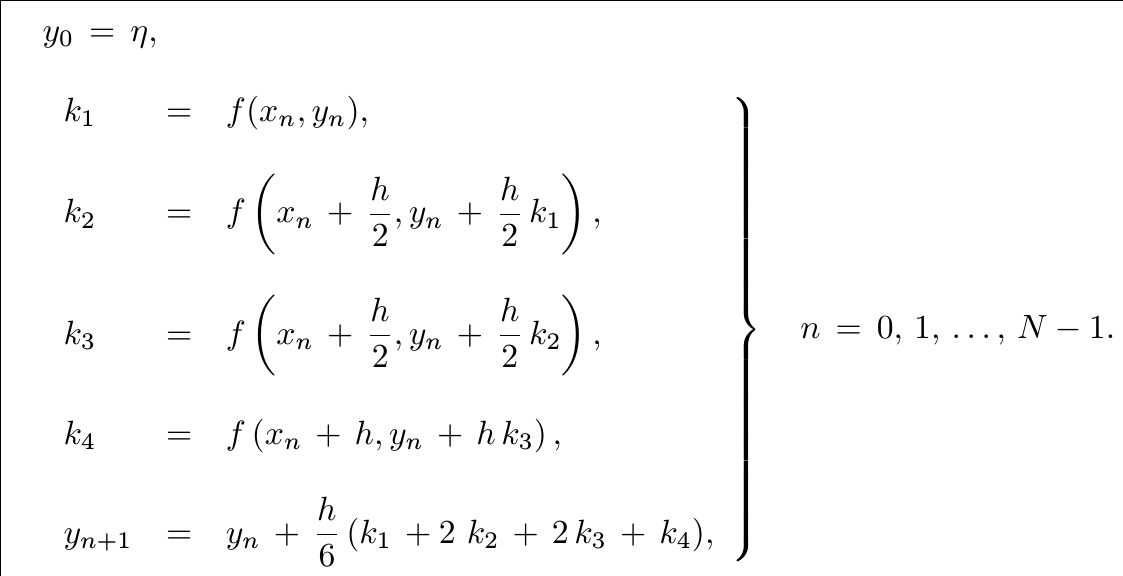
\includegraphics[width=0.9\linewidth]{tema4/R-K-clasico}
%   \end{center}
% \end{example}

% \section{Métodos multipaso}
% \label{sec:metodos-multipaso}

% Los métodos numéricos de $k$ son aquellos en los que, para calcular
% $y_{n+k}$ (una aproximación de $y(t_{n+k})$), se utilizan
% aproximaciones de la solución en $k$ etapas de tiempo anteriores,
% \begin{equation*}
%   y_n,\  y_{n+1},\ \dots, y_{n+k-1} \quad \longmapsto \quad y_{n+k}.
% \end{equation*}
% Específicamente:
% \begin{definition}
%   Un método numérico (lineal) de $k$ pasos para aproximar la solución
%   de~(\ref{eq:pvi}) es todo aquel en el que la solución en
%   la etapa $n+k$ viene dada por una expresión recursiva de la forma:
%   \begin{align}
%     \label{eq:metodo-multipaso}
%     \ddt y_{n+k}=&\sum_{j=0}^k \beta_j f(t_{n+j},y_{n+j}), \quad
%     n=0,...,N-k, \intertext{donde $\ddt y_{n+k}$ es un aproximación
%       de $y'(t_{n+k})$ usando un cociente incremental con $k$ pasos:}
%     \ddt
%     \label{eq:cociente-incremental-multipaso}
%     y_{n+k}&=\frac{1}{h}\sum_{j=0}^k\alpha_j y_{n+j}.
%   \end{align}
% \end{definition}
% En las expresiones anteriores, $\alpha_j, \beta_j\in\Rset$, con
% $\alpha_k\neq 0$. Por simplificar, supondremos $$\alpha_k=1$$ (lo que
% equivale a dividir todos los coeficientes por $\alpha_k$).

% Por ejemplo, los métodos de Euler (explícito e implícito) y el esquema
% de Crank-Nicolson~(\ref{eq:crank-nicolson-2}) son métodos de este tipo
% con un único paso $k=1$. Más adelante se muestran algunos métodos con
% $k>1$.
% Con el fin de abreviar, con frecuencia usaremos la siguiente notación:
% $$f_n=f(\tn,\yn).$$

% Puesto que en un método de $k$ pasos del
% tipo~(\ref{eq:metodo-multipaso}) se necesitan $k$ aproximaciones
% previas para calcular $y_{n+k}$, en la primera iteración ($n=0$) es
% necesario disponer de $k$ valores de arranque, $y_0$, $y_1$, ...,
% $y_{k-1}$ (que determinarán $y_k$). Pero en~(\ref{eq:pvi}) sólo
% contamos con un dato inicial, $\ycero$, de forma que necesitaremos
% usar algún método numérico para aproximar $y_1$, $y_2$, ...,
% $y_{k-1}$. Habitualmente se usarán métodos de un paso, con especial
% cuidado en que el orden de estos métodos sea (al menos) igual al
% del método multipaso (pues, de otra forma, perderíamos calidad en la
% aproximación inicial).

% \begin{enumerate}
% \item Si $\beta_k=0$, el método se dice \emph{explícito}. El término
%   $f_{n+k}=f(t_{n+k},y_{n+k})$ no aparece en el segundo miembro
%   de~(\ref{eq:metodo-multipaso}) del método multipaso, en
%   consecuencia, usando~(\ref{eq:cociente-incremental-multipaso}),
%   $y_{n+k}$ puede expresarse explícitamente:
%   \begin{equation*}
%     y_{n+k}=
%     h\sum_{j=0}^{k-1} \beta_j f_{n+j}-\sum_{j=0}^{k-1}\alpha_j y_{n+j}.
%   \end{equation*}
% \item Si $\beta_k\neq 0$, el método se dice \emph{implícito}. No podemos
%   expresar explícitamente el término $y_{n+k}$ y, en cada paso,
%   para calcular este término será necesario resolver la ecuación (no
%   lineal, en general):
%   \begin{equation*}
%     y_{n+k} - \beta_k f(t_{n+j},y_{n+j})=
%      h\sum_{j=0}^{k-1} \beta_j f(t_{n+j},y_{n+j})- \sum_{j=0}^{k-1}\alpha_j y_{n+j} .
%   \end{equation*}
%   Para resolver este tipo de ecuaciones existen distintas
%   posibilidades, las más habituales de las cuales son el método de
%   aproximaciones sucesivas (o de punto fijo) y el método de Newton
%   (para asegurar la convergencia, de estos métodos, será necesario
%   imponer hipótesis adicionales a $f$).
% \end{enumerate}

% \subsection*{Construcción de métodos multipaso lineales}

% Para deducir algunos métodos multipaso utilizaremos la formulación
% integral de la ecuación diferencial
% $$
% y'=f(t,y),
% $$
% es decir fijados $t,t^*\in[a,b]$ escribimos
% \begin{equation*}
%   y(t^*)-y(t) = \int_{t}^{t^*} f(x,y(x))\, dx.
% \end{equation*}
% Para cada $n=0,...,N-k$, elegimos $t=x_{n+k-1}$ y $t^*=x_{n+k}$ y
% denotando $y_{n+j}\approx y(t_{n+j})$ a las aproximaciones que
% deseamos calcular,  ponemos en práctica la siguiente idea:
%   % realizar, en esta formulación integral las siguiente
% % aproximación:
% \begin{enumerate}
% \item Elegir $t=x_{n+k-1}$ y $t^*=x_{n+k}$
% % \item Elegir $t$ y $t^*$ adecuadamente.
% % \item Sustituir la función $F(t)=f(t,y(t))$ por su polinomio de
% %   interpolación de Lagrange, $P(t)$, en los nodos $t_n,\ t_{n+1},\
% %   \dots, t_{n+k}$.
% \item Sustituir la función $F(x)=f(x,y(x))$ por su polinomio de
%   interpolación de Lagrange, $P(x)$, en un soporte
%   $S\subset \{t_{n+j}\}_{j=0}^k$ adecuado:%  interpola los valores
%   % $\{f(t_{n+j},y_{n+j})\}_{j=0}^k$.
%   \begin{enumerate}
%   \item Métodos de \emph{\AB}:
%     \begin{equation*}
%       S= \{t_{n+j}\}_{j=0}^{k-1}.
%     \end{equation*}
%     Como veremos, se trata de métodos explícitos, pues en la
%     aproximación no aparece el término
%     $f(t_{n+k},y_{n+k})$.
%   \item  Métodos de \emph{\AM}:
%     \begin{equation*}
%       S= \{t_{n+j}\}_{j=0}^{k},
%     \end{equation*}
%     dando lugar a métodos implícitos.
%   \end{enumerate}
% \end{enumerate}

% \begin{example}[Método de \AB de dos pasos (orden 2)]
%   \label{sec:AB-dos-pasos}
%   Consideremos la siguiente expresión integral:
%   \begin{equation}
%    \label{eq:tema4:8}
%    y(t_{n+2})-y(t_{n+1}) \approx \int_{t_{n+1}}^{t_{n+2}} P(t)\,dt,
%   \end{equation}
%   donde $P(t)$ es el polinomio de interpolación de $F(t)=f(t,y(t))$ en
%   $t_n$ y $t_{n+1}$. Para construirlo, podemos usar la fórmula de
%   diferencias dividas de Newton o bien la fórmula de Lagrange. En este
%   último caso:
%   \begin{equation*}
%    P(t)=F(t_n)\frac{t-t_{n+1}}{t_n-t_{n+1}} +
%    F(t_{n+1})\frac{t-t_{n}}{t_{n+1}-t_{n}}.
%   \end{equation*}
%   Con un simple cálculo (puede ser útil el cambio de variable $t =
%   t_{n+1}+h\,s$, que transforma $t\in [t_{n+1},t_{n+2}]$ en $s\in [0,1]$)
%   el segundo miembro de~(\ref{eq:tema4:8}) resulta:
%   \begin{equation*}
%   \int_{t_{n+1}}^{t_{n+2}} P(t)\,dt = \frac{h}{2} \big[
%   3(f(t_{n+1},y(t_{n+1})) - f(t_{n},y(t_{n})) \big].
%   \end{equation*}
%   Planteamos, por tanto, la siguiente aproximación: dados $y_n$,
%   $y_{n+1}$, calcular $y_{n+2}$ como solución de la
%   siguiente fórmula de recurrencia:
%   \begin{equation}
%     \tag{AB2}
%     \label{eq:AB2}
%     y_{n+2}-y_{n+1} = \frac{h}{2} \big[
%     3f(t_{n+1},y_{n+1}) - f(t_{n},y_{n}) \big],
%   \end{equation}
%   de donde, para cada $n=0,...,N-2$ podemos obtener explícitamente el
%   valor $y_{n+2}$.

%   El valor $y_0$ se puede obtener a partir del dato inicial $\ycero$,
%   mientras que para el cálculo de $y_1$ será necesario utilizar un
%   método numérico de un paso. Se puede demostrar que este método
%   de \AB tiene orden 2, por tanto el método para inicializar debe
%   tener el mismo orden (por ejemplo, Euler--Cauchy o Euler mejorado).
% \end{example}

% \begin{example}[Método de \AM de dos pasos (orden 2)]
%   Si consideramos la ecuación integral (\ref{eq:tema4:8}) pero
%   definimos $P(t)$ como el polinomio de interpolación de
%   $f(t,y(t))$ en $\{t_n,t_{n+1},t_{n+2}\}$, obtenemos el método
%   de \AM de dos pasos. Procediendo como en el ejemplo anterior (lo que
%   se deja como ejercicio) se obtiene:
%   \begin{equation}
%     \tag{AM2}
%     \label{eq:AM2}
%       y_{n+2}-y_{n+1} = \frac{h}{12} \big[
%       5f(t_{n+2},y_{n+2}) + 8 f(t_{n+1},y_{n+1}) - f(t_{n},y_{n}) \big].
%   \end{equation}
%   Se puede demostrar que el orden de este método es igual a
%   $2$. Puesto que se trata de un método implícito, en principio será
%   necesario usar algún método numérico (por ejemplo, iteraciones de
%   punto fijo) en cada instante $\tn$ para hallar $y_{n+2}$.
% \end{example}

% \begin{example}[Método predictor-corrector~(\ref{eq:AB2})--(\ref{eq:AM2})]
%   Con frecuencia, los métodos de \AB y \AM del mismo orden se suelen
%   combinar para dar lugar a nuevos métodos numéricos. La idea es, en
%   cada etapa $t_n$:
%   \begin{enumerate}
%   \item Utilizar el método de \AB para obtener, de forma explícita una
%     primera aproximación (predicción) de $y_{n+k}$.
%   \item Utilizar la predicción obtenida para aproximar
%     $f(t_{n+k},y_{n+k})$ y así calcular, mediante el método de \AM,
%     una nueva aproximación (corrección) de $y_{n+k}$.
%   \end{enumerate}

%   En el caso~(\ref{eq:AB2})--(\ref{eq:AM2}) cada etapa del método
%   queda:
%   \begin{equation*}\left\{
%       \begin{aligned}
%         y^*_{n+2} &= y_{n+1} + \frac{h}{2} \big[ 3f(t_{n+1},y_{n+1}) -
%         f(t_{n},y_{n}) \big] \quad \text{(predicción),}
%         \\
%         y_{n+2} &= y_{n+1} + \frac{h}{12} \big[ 5f(t_{n+2},y^*_{n+2})
%         + 8 f(t_{n+1},y_{n+1}) - f(t_{n},y_{n}) \big] \quad
%         \text{(corrección).}
%       \end{aligned}\right.
%   \end{equation*}
%   Así obtenemos un método explícito que saca partida a las
%   características de los esquemas de \AB y AM.
%   \end{example}
%%% Local Variables:
%%% mode: latex
%%% TeX-master: "../apuntes-MNII.tex"
%%% End:
